\documentclass[../DC2017114Bouma.tex]{subfiles}
\begin{document}
\graphicspath{{02_Material/img/}}
%% New chapter
\renewcommand{\chaptermark}[1]{\markboth{\thechapter.\ #1}{}}
\renewcommand{\sectionmark}[1]{\markright{#1}{}}
\pagestyle{fancyreport}
\cleartooddpage
\pagestyle{fancyreport}
\chapter{Mechanical Systems with Unilateral Constraints and Spatial Friction}\label{ch:model}
\nomenclature[F]{$\Db$}{Delassus matrix}
In this chapter several modeling approaches of mechanical systems with unilateral constraints and spatial friction are presented. First a general representation of such a system is given, which is followed by sections introducing several formulations of the contact and friction laws in these systems. First a complementarity problem formulation is given, which is a complete and often used formulation for mechanical systems with unilateral constraints. From the complementarity formulation a hybrid system formulation is derived, which although less complete is a more intuitive formulation from a control point-of-view.
\section{General system definition}
For mechanical systems a set of contact points $\iota\in\{\iota_1,\iota_2,...,\iota_c\}$ is defined, with $c$ being the number of considered contact points. A set $\Ic_{\text{cl}}$ is defined as the set of $c_{\text{cl}}$ closed contact points, such that a contact $\iota\in\Ic_{\text{cl}}$ has closed a unilateral constraint. The set of contact points in open contact is defined as $\Ic_{\text{op}} := \{\iota\ |\ \iota\notin\Ic_{\text{cl}}\}$. When a unilateral constraint is activated at a nonzero velocity impact happens, meaning a jump in the velocity will appear. Therefore the generalized velocity $\dot{\qb}$ is not continuously defined over the entire domain of a trajectory with impacts. Therefore $\xib:=\dot{\qb}$ is defined, except at impact-times $\tau_i$. Here $i$ is a counter for unilateral constraint activations where $i\in \{1,2,...,N\}$, with $N$ the amount of jumps in a trajectory. $h_{n,\iota}$ is the normal contact distance and $\zeta_{n,\iota}$ and $\zetab_{t,\iota}$ represent the relative velocities in normal and tangential direction,  respectively. 

In Figure~\ref{fig:contactplanes} a body and a fixed world surface are illustrated. A contact point $\iota$ is defined on the body, on which a plane tangent to the surface of the body is spanned. On the normal direction of this plane, the contact distance $h_{n,\iota}(\qb)$ is defined. This is the distance between the contact point and the surface that it can make contact with. By taking the time derivative of $h_{n,\iota}(\qb)$, the relative normal velocity of contact point $\iota$ is found to be
\begin{align}
\zeta_{n,\iota} = \frac{\partial h_{n,\iota}}{\partial\qb}\frac{\text{d}\qb}{\text{d} t} = \wb_{n,\iota}^T\dot{\qb},
\end{align}
\nomenclature[C]{$\iota$}{The contact point counter}%
\nomenclature[C]{$i$}{The macro-event counter}%
\nomenclature[P]{$c$}{The number of contact points}%
\nomenclature[P]{$N$}{The number of events}%
\nomenclature[F]{$\wb_{n,\iota}$}{The normal jacobian of contact point $\iota$}%
\nomenclature[F]{$\Wb_{t,\iota}$}{The tangential jacobian of contact point $\iota$}%
\nomenclature[A]{$(.)_{\text{cl}}$}{The closed-contact mode sub/superscript}%
\nomenclature[A]{$(.)_{\text{op}}$}{The open-contact mode sub/superscript}%
\nomenclature[A]{$(.)_{\text{sl}}$}{The slip-contact mode sub/superscript}%
\nomenclature[A]{$(.)_{\text{st}}$}{The stick-contact mode sub/superscript}%
\nomenclature[P]{$\Ic$}{A set of contact points}%
\nomenclature[V]{$\qb$}{The generalized coordinates}%
\nomenclature[V]{$\xb$}{The state coordinates}%
\nomenclature[V]{$\ub$}{The input}%
\nomenclature[V]{$\tau$}{The nominal event time}%
\nomenclature[V]{$t$}{Regular time}%
\nomenclature[V]{$\xib$}{The generalized coordinates defined on the continuous segments of a trajectory}%
\nomenclature[V]{$h_{n,\iota}$}{Contact distance of contact point $\iota$}%
\nomenclature[V]{$\zeta_{n,\iota}$}{Normal velocity of contact point $\iota$}%
\nomenclature[V]{$\zetab_{t,\iota}$}{Tangential velocity of contact point $\iota$}%
with $\wb_{n,\iota}$ representing the Jacobian of the normal velocity $\zeta_{n,\iota}$. The relative tangential velocity $\zetab_{t,\iota}$ is defined in the tangent plane of $\iota$, and thus lies perpendicular to $\zeta_{n,\iota}$. Using the tangential velocity jacobian $\Wb_{t,\iota}$, the relative tangential velocity is defined as
\begin{align}
\zetab_{t,\iota} = \Wb_{t,\iota}^T\dot{\qb}.
\end{align}

\begin{figure}[h]
\centering
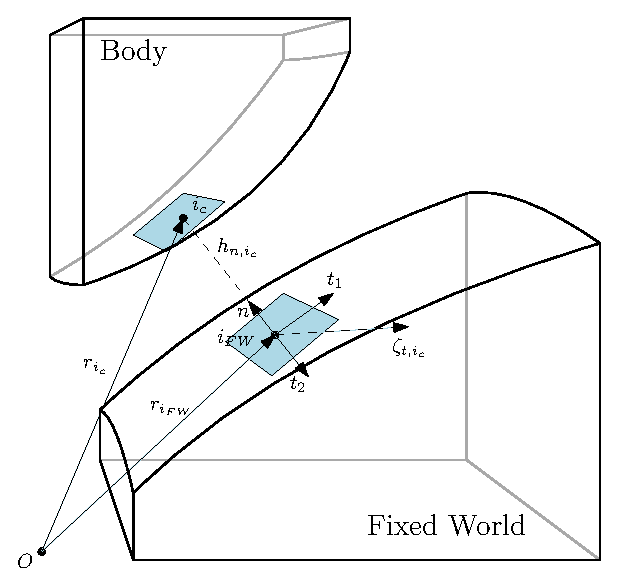
\includegraphics[width=.5\textwidth]{contactplanes.eps}\caption{An illustration of a body impacting the fixed world. A contact point $\iota$ is defined on the body, which can make contact with the fixed world at $i_{FW}$. The points $\iota$ and $i_{FW}$ are connected by a line which is perpendicular to their respective bodies, which is used to define the contact distance $h_{n,\iota}$ and normal contact velocity $\zeta_{n,\iota}$. In the plane tangent to the body's surface, the tangential contact velocity $\zetab_{t,\iota}$ is defined.} \label{fig:contactplanes}
\end{figure}

Then, the continuous dynamics of a mechanical system with unilateral constraints and spatial friction are of the form
\begin{align}
&\Mb(\qb)\dot{\xib} + \Cb(\qb,\xib) = \Sb(\qb)\ub + \sum_{\iota\in\Ic_{\text{cl}}}\left(\wb_{n,\iota}(\qb)\lambda_{n,\iota} + \Wb_{t,\iota}(\qb)\lambdab_{t,\iota} \right), \label{eq:appcont1}\\
&\text{(Contact Law)},\label{eq:appcont2}\\
&\text{(Friction Law)},\label{eq:appcont3}
\end{align}
\nomenclature[V]{$\lambda_{n,\iota}$}{The normal reaction force of contact point $\iota$}%
\nomenclature[V]{$\lambdab_{t,\iota}$}{The tangential reaction force of contact point $\iota$}%
\nomenclature[V]{$\Lambda_{n,\iota}$}{The normal impulsive reaction force of contact point $\iota$}%
\nomenclature[V]{$\Lambdab_{t,\iota}$}{The tangential impulsive reaction force of contact point $\iota$}%
\nomenclature[F]{$\Mb$}{The mass matrix}%
\nomenclature[F]{$\Cb$}{The column containing centripedal, Coriolis and gravitational effects}%
\nomenclature[F]{$\Sb$}{The matrix containing generalized directions of the actuator forces}%
with $\qb,\xib\in\Rbb^{n}$ and $\ub\in\Rbb^m$. Here $\Mb(\qb)\in\Rbb^{n\times n}$ is the mass matrix of the system, $\Cb(\qb,\xib)\in\Rbb^{n}$ contains the centripetal, Coriolis and gravitational forces in the system and $\Sb(\qb)\in\Rbb^{n\times m}$ represents the generalized directions of the forces. $\lambda_{n,\iota}\in\Rbb$ and $\lambdab_{t,\iota}\in\Rbb^{2}$ are the normal and tangential reaction forces, respectively, of contact point $\iota$ with $\wb_{n,\iota}\in\Rbb^{n}$ and $\Wb_{t,\iota}\in\Rbb^{n\times 2}$ the corresponding reaction force jacobians. When a contact point activates a unilateral constraint, impulsive dynamics can cause the state of the system to jump. These dynamics are of the form

\begin{align}
&\Mb(\qb)(\xib^+ - \xib^-) = \sum_{\iota\in\Ic_{\text{cl}}}\left( \wb_{n,\iota}(\qb)\Lambda_{n,\iota} + \Wb_{t,\iota}(\qb)\Lambdab_{t,\iota}\right), \label{eq:appimp1}\\
&\text{(Impulsive Contact Law)},\label{eq:appimp2}\\
&\text{(Impulsive Friction Law)}.\label{eq:appimp3}
\end{align}
Here $\Lambda_{n,\iota}$ and $\Lambdab_{t,\iota}$ the normal and tangential impulsive reaction forces, respectively, of contact point $\iota$. These dynamics are impulsive, and happen at one instance in time. The $^-$ superscript indicates the ante-event state and the $^+$ superscript indicates the post-event state. In the following sections three different methods of describing the contact and friction laws are presented. First a complementarity problem formulation of mechanical systems with unilateral constraints is given, from which later a proximal point formulation and a hybrid system formulation are derived. For more information on modeling of multibody systems one can refer to \cite{Leine2008} and \cite{Wouw2016}. \textbf{Modes vs states}

\section{Complementarity problem formulation}\label{sec:comp}
\subsection{Signorini's contact law and Poisson's impact law}
To describe the normal contact between rigid bodies Signorini's contact law is used. Since the bodies are impenetrable and reaction forces caused by contact cannot prevent the bodies from seperating, both the contact distance $h_{n,\iota}$ and $\lambda_{n,\iota}$ cannot become negative. Two situations are possible

\begin{enumerate}
\item $h_{n,\iota}=0\ \wedge\ \lambda_{n,\iota} \geq 0$ (closed-contact)
\item $h_{n,\iota}>0\ \wedge\ \lambda_{n,\iota} = 0$ (open-contact)
\end{enumerate}

These situations are illustrated in Figure~\ref{fig:signorinicontact}, where it can be seen that the two situations are orthogonal. This behavior can be summarized in the complementarity condition

\begin{align}
0\leq h_{n,\iota}\ \bot\ \lambda_{n,\iota} \geq 0,\label{eq:signorini}
\end{align}

where the symbol $\bot$ is used to express the orthogonality between $h_{n,\iota}$ and $\lambda_{n,\iota}$. The complementarity condition in \eqref{eq:signorini} is called Signorini's contact law.
\begin{figure}[h]
\centering
\begin{subfigure}{0.3\textwidth}
\centering
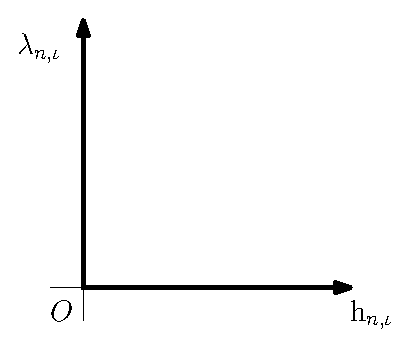
\includegraphics[width=\linewidth]{signorinicontact.eps}
\caption{Signorini's contact law.}\label{fig:signorinicontact}
\end{subfigure}
\qquad
%\begin{subfigure}{0.3\textwidth}
%\centering
%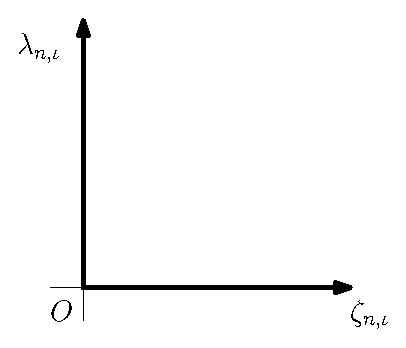
\includegraphics[width=\linewidth]{signoriniforce.eps}
%\caption{Signorini's force law.}\label{fig:signoriniforce}
%\end{subfigure}
%\quad
\begin{subfigure}{0.3\textwidth}
\centering
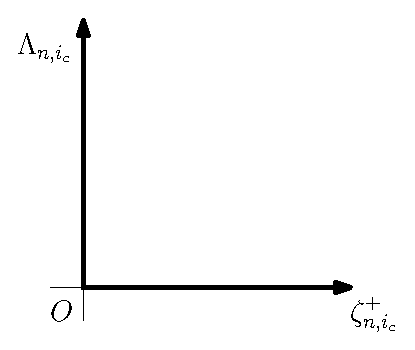
\includegraphics[width=\linewidth]{poissonimpact.eps}
\caption{Poisson's impact law without restitution.}\label{fig:poissonimpact}
\end{subfigure}
\caption{}
\end{figure}
When contact happens at nonzero velocity, impact occurs. Newton's impact law is used to describe this impact. Newton's law of impact is defined as
\begin{align}
\zeta^+_{n,\iota} = -e_{n,\iota}\zeta^-_{n,\iota},\text{ when }h_{n,\iota}=0,\ \dot{h}_{n,\iota}<0.
\end{align}
\nomenclature[P]{$e_{n,\iota}$}{}%
\nomenclature[P]{$e_{t,\iota}$}{}%
In this work the coefficient of restitution $e_{n,\iota}$ is assumed to be $0$, describing a completely inelastic contact. For closed contact an impact law can be defined that relates the impulsive contact force $\Lambda_{n,\iota}$ to the post-impact normal velocity $\zeta_{n,\iota}$. When considering multi-contact systems, when a contact is closed two situations can occur:
\begin{enumerate}
\item $\Lambda_{n,\iota} > 0\ \wedge\ \zeta^+_{n,\iota} = 0$ (impact)
\item $\Lambda_{n,\iota} = 0\ \wedge\ \zeta^+_{n,\iota} \geq 0$ (no impact)
\end{enumerate}
The second case can occur when a contact point other than $\iota$ makes impact. The situations described above are illustrated in Figure~\ref{fig:poissonimpact}, where again the orthogonality can be observed. The behavior is written into the complementarity condition
\begin{align}
0\leq \zeta^+_{n,\iota}\ \bot\ \Lambda_{n,\iota} \geq 0,\quad  \qquad \forall \iota\in\Ic_{\text{cl}},\label{eq:poisson}
\end{align}
with $\Ic_{\text{cl}}$ the set of closed contacts. The complementarity condition \eqref{eq:poisson} is called Poisson's impact law. Note that the impact law is defined on velocity level, whereas the contact law is defined on position level.

\subsection{Coulomb's friction law}
Coulomb's friction law is often used to describe dry friction in mechanical systems. When considering 3-dimensional environments, Coulomb's friction law is defined as 
\begin{align}
||\lambdab_{t,\iota}||\ \in\ \left\{ \begin{array}{ll}
||\lambdab_{t,\iota}||\leq\mu_{\iota}\lambda_{n,\iota}, &\text{if }||\zetab_{t,\iota}||=0\\
||\lambdab_{t,\iota}|| = \mu_{\iota}\lambda_{n,\iota}, &\text{if }||\zetab_{t,\iota}||>0
\end{array}\right.,\label{eq:frictionlen}
\end{align}
\nomenclature[P]{$\mu_{\iota}$}{The friction coefficient of contact point $\iota$}%
with $\mu_{\iota}$ the friction coefficient of contact point $\iota$, and since friction is considered isotropic
\begin{align}
\zetab_{t,\iota} = -\kappa_{\iota}\SgnSp(\lambdab_{t,\iota}),\label{eq:frictiondir}
\end{align}
\nomenclature[P]{$\kappa_{\iota}$}{Magnitude of the tangential velocity of contact point $\iota$}
with $\kappa_{\iota}>0$ and
\begin{equation}
\SgnSp(a) = \left\lbrace\begin{array}{ll}
\frac{a}{||a||} & a \neq 0\\
0 & a = 0
\end{array},\right.
\end{equation}
for some vector $a$ as defined in \cite{Studer2006}. \eqref{eq:frictionlen} can be considered as a relation between the magnitude of the tangential velocity $\zetab_{t,\iota}$ and the reaction friction force $\lambdab_{t,\iota}$. \eqref{eq:frictiondir} can be considered as a relation between the direction of $\zetab_{t,\iota}$ and $\lambdab_{t,\iota}$, namely that $\zetab_{t,\iota}$ and $\lambdab_{t,\iota}$ are always in opposite directions. The constant $\kappa_{\iota}$ can then be interpreted as the magnitude of the tangential velocity. Coulomb's friction law is illustrated in Figure~\ref{fig:coulombfriction}. In Figure~\ref{fig:coulombort} the same law is illustrated, but now as orthogonal vectors. As noticed earlier, this is convenient for writing the law in a complementarity form.

\begin{figure}[h]
\centering
\begin{subfigure}{0.38\textwidth}
\centering
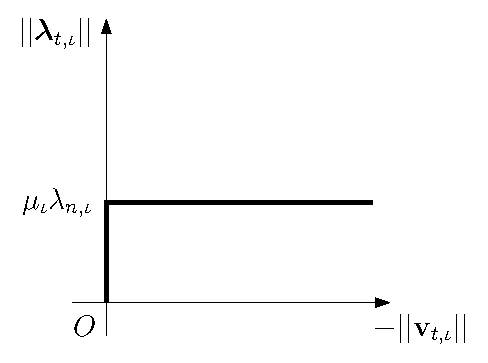
\includegraphics[width=\linewidth]{coulombfriction.eps}\caption{Coulomb's friction law.}\vspace{1.25cm}\label{fig:coulombfriction}
\end{subfigure}
\qquad
\begin{subfigure}{0.3\textwidth}
\centering
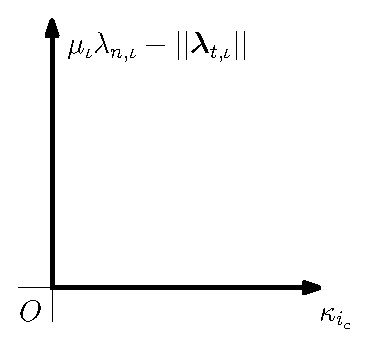
\includegraphics[width=\linewidth]{coulombort.eps}\caption{Coulomb's friction law as orthogonal vectors. $\kappa_{\iota}$ is defined as the magnitude of the tangential velocity $\zetab_{t,\iota}$.}\label{fig:coulombort}
\end{subfigure}
\caption{}
\end{figure}

The complementarity formulation of the Coulomb's law is therefore defined as

\begin{align}
&0\leq \left(\mu_{\iota}\lambda_{n,\iota} - ||\lambdab_{t,\iota}||\right)\ \bot\ \kappa_{\iota} \geq 0,\label{eq:coulomb1}\\
&\zetab_{t,\iota} = -\kappa_{\iota}\SgnSp(\lambdab_{t,\iota}).\label{eq:coulomb2}
\end{align}

\eqref{eq:frictiondir} is rewritten to \eqref{eq:coulomb2} to avoid singularity problems for $||\lambdab_{t,\iota}|| = 0$. For the impulsive behavior of the friction law Newton's impact law is used to define the tangential post-impact velocity as
\begin{align}
\zetab^+_{t,\iota} = -e_{t,\iota}\zetab^-_{t,\iota},
\end{align}
where in this work $e_{t,\iota}=0$ is assumed. Then, similarly to the non-impulsive case, the impulsive Coulomb's friction law can be defined as
\begin{align}
&0 \leq (\mu\Lambda_{n,\iota} - ||\Lambdab_{t,\iota}||)\ \bot\ \kappa_{\iota} \geq 0. \qquad \forall \iota\in\Ic_{\text{cl}},\label{eq:coulombimp1}\\
&\zetab_{t,\iota}^+ = \kappa_{\iota}\SgnSp(\Lambdab_{t,\iota}),\qquad \forall \iota\in\Ic_{\text{cl}}.\label{eq:coulombimp2}
\end{align}
Note that just as the contact case, the impulsive friction law only holds for closed contacts.
\subsection{System dynamics with contact and friction law}
The flow dynamics are then described by
\begin{align}
&\Mb(\qb)\dot{\xib} + \Cb(\qb,\xib) = \Sb(\qb)\ub + \sum_{\iota\in\Ic_{\text{cl}}}\left(\wb_{n,\iota}(\qb)\lambda_{n,\iota} + \Wb_{t,\iota}(\qb)\lambdab_{t,\iota} \right), \label{eq:ncpcontact1}\\
&0\leq h_{n,\iota}\ \bot\ \lambda_{n,\iota} \geq 0,\label{eq:ncpcontact2}\\
&0\leq \left(\mu\lambda_{n,\iota} - ||\lambdab_{t,\iota}||\right)\ \bot\ \kappa_{\iota} \geq 0,\label{eq:ncpcontact3}\\
&\zetab_{t,\iota} = -\kappa_{\iota}\SgnSp(\lambdab_{t,\iota}),\label{eq:ncpcontact4}
\end{align}
with 
\begin{align}
&h_{n,\iota} = \wb_{n,\iota}^T(\qb)\qb,\label{eq:h}\\
&\zeta_{n,\iota}(\qb) = \wb^T_{n,\iota}(\qb) \xib,  \label{eq:zetan}\\
&\zetab_{t,\iota}(\qb) = \Wb^T_{t,\iota}(\qb) \xib. \label{eq:zetab}
\end{align}
The discrete dynamics, which take place when a contact point goes through an event, are described by
\begin{align}
&\Mb(\qb)(\xib^+ - \xib^-) = \sum_{\iota\in\Ic_{\text{cl}}}\left( \wb_{n,\iota}(\qb)\Lambda_{n,\iota} + \Wb_{t,\iota}(\qb)\Lambdab_{t,\iota}\right), \label{eq:ncpimpact1}\\
&0\leq \zeta_{n,\iota}^+\ \bot\ \Lambda_{n,\iota} \geq 0, \qquad \forall \iota\in\Ic_{\text{cl}},\label{eq:ncpimpact2}\\
&0 \leq (\mu\Lambda_{n,\iota} - ||\Lambdab_{t,\iota}||)\ \bot\ \kappa_{\iota} \geq 0. \qquad \forall \iota\in\Ic_{\text{cl}},\label{eq:ncpimpact3}\\
&\zetab_{t,\iota}^+ = -\kappa_i\SgnSp(\Lambdab_{t,\iota}),\qquad \forall \iota\in\Ic_{\text{cl}},\label{eq:ncpimpact4}
\end{align}
with 
\begin{align}
&\zeta^+_{n,\iota}(\qb) = \wb^T_{n,\iota}(\qb) \xib^+,\\
&\zetab^+_{t,\iota}(\qb) = \Wb^T_{t,\iota}(\qb) \xib^+.\label{eq:ncpimpactend}
\end{align}

\section{Hybrid system formulation}
In this section the dynamics of the complementarity system defined in Section~\ref{sec:comp} is written to a hybrid formulation, resulting in a hybrid framework for mechanical systems with unilateral constraints and spatial friction. The hybrid system formulation only holds for trajectories where only the contact points activating a guard function are allowed to change mode, i.e. no superfluous contacts. More information on the considered trajectories in this work is given in Section~\ref{app:trajectories}.

\subsection{Hybrid systems with impulsive effects}\label{sec:2hyb}
According to \cite{Haddad2006} an impulsive dynamical system can be described by a hybrid system with impulsive effects. This makes it a valid framework for mechanical systems with unilateral constraints and spatial friction. The notation given in \cite{Haddad2006} is convenient from a tracking point-of-view, in that only the dynamics encountered during the trajectory need to be described. A hybrid system with impulsive effects consists of three elements:
\begin{enumerate}
\item Continuous dynamics, a continuous-time differential equation which defines the behavior of the system in between events
\item Discrete dynamics, which defines the way the state of the system is reset during events
\item Reset sets, which is a criterion to decide when the state of the system is to be reset
\end{enumerate}

Therefore, a hybrid system with impulsive effects is given by
\begin{equation}
\begin{array}{ll}
\dot{\xb}(t,i) =\fb_i(\xb(t,i),\ub(t,i),t),& \xb(t,i),\ub(t,i)\notin D_i\\
\xb(t,i) = \gb_i(\xb(t,i-1),\ub(t,i-1),t),& \xb(t,i-1),\ub(t,i-1)\in D_i
\end{array}\label{eq:hybimp}
\end{equation}
\nomenclature[F]{$\fb$}{A nonlinear continuous function}%
\nomenclature[F]{$\gb$}{A jump map}%
\nomenclature[F]{$D$}{A discrete event set}%
\nomenclature[F]{$\gamma$}{A flow guard function}%
\nomenclature[F]{$\Gamma$}{An impulsive guard function}%
\nomenclature[F]{$\alphab$}{The nominal reference trajectory}%
\nomenclature[F]{$\mub$}{The nominal reference input}%
with $\xb(t,i)\in\Rbb^{n(i)}$, $\ub(t,i)\in\Rbb^{m(i)}$, $\fb_i(t,i)\ :\ \Rbb^{n(i)}\ \times\ \Rbb^{m(i)}\ \times\ \Rbb\rightarrow \Rbb^{n(i)}$. Note that the state dimension $n(i)$ and the input dimension $m(i)$ can vary in different modes $i$. For the difference equation we have $\gb_i\ :\ \Rbb^{n(i-1)}\ \times\ \Rbb^{m(i-1)}\ \times\ \Rbb\rightarrow \Rbb^{n(i)}$. The set $D_i = D_i(t) := \{\xb(t,i)\in\Rbb^{n(i)},\ \ub(t,i)\in\Rbb^{m(i)}\ |\ \gamma^{=}_i(\xb^{\wedge},\ub^{\wedge},t) = 0, \ \gamma^{\geq}_i(\xb^{\wedge},\ub^{\wedge},t) \geq 0\}$, where $\gamma^{=}_i$ and $\gamma^{\geq}_i$ are some sets of guard functions that are activated at event $i$, and $\xb^{\wedge}$,$\ub^{\wedge}$ are some virtual state and input that are not necessarily physically realistic.

The dynamics given in \eqref{eq:hybimp} will be used to describe a tracking problem for mechanical systems with unilateral constraints and spatial friction. A nominal state-input trajectory is considered consisting of absolutely continuous segments $(\alphab(t,i),\mub(t,i))$, with $t\in\left[\tau_i,\tau_{i+1}\right]$ and $i\in\{0,1,...,N\}$ the event counter. $\alphab(t,i)$ and $\mub(t,i)$ are the nominal state and input, respectively, that define the nominal trajectory with $N$ events. $\tau_i$ is referred to as the nominal event time of event $i$ and $t$ is referred to as regular time. Every segment of the nominal trajectory $(\alphab(t,i),\mub(t,i))$ and every event $i\in\{0,1,...,N\}$ satisfy the dynamics in \eqref{eq:hybimp}, where an event happens when $(\alphab(t,i),\mub(t,i))$ enters $D_{i+1}$. Such a nominal trajectory existing of absolutely continuous segments experiencing events according to \eqref{eq:hybimp} is illustrated in Figure~\ref{fig:2exampletraj}.

In \ref{fig:2example} an example trajectory of a block pushing towards a surface is illustrated. The block has two contact points on its edges $i_1$ and $i_2$. It starts with both contact points in open contact as can be seen in Figure~\ref{fig:2example1}. The flow is described by $\dot{\alphab}(t,0) = \fb_0(\alphab(t,0),\mub(t,0),t)$ for $t\in[t_0,\tau_1]$. Then $i_2$ makes impact with the surface at $\tau_1$, causing a jump in the state and a change in continuous dynamics $\dot{\alphab}(t,1) = \fb_1(\alphab(t,1),\mub(t,1),t)$ for $t\in[\tau_1,\tau_2]$. This is illustrated in Figure~\ref{fig:2example2}, where $i_2$ is in closed contact and slipping over the contact surface. At $\tau_2$, $i_1$ makes impact as well causing another jump and another change in continuous dynamics. The block now has both contact points slipping over the contact surface. After this both contact points release contact one by one. Since there are no impulsive forces present in this transition, the state does not jump when a contact point releases. However, a jump in the time-derivate of the state is possible, which makes these transitions continuous but nonsmooth.

\begin{figure}[h]
\centering
\begin{subfigure}[b]{0.17\textwidth}
\centering
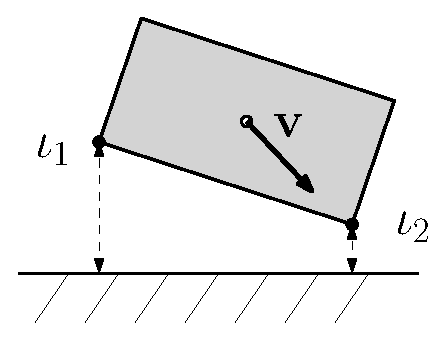
\includegraphics[width=\textwidth]{example1.eps}
\caption{$i_1,i_2\in\Ic_{\text{op}}$}
\label{fig:2example1}
\end{subfigure}
\quad
\begin{subfigure}[b]{0.17\textwidth}  
\centering 
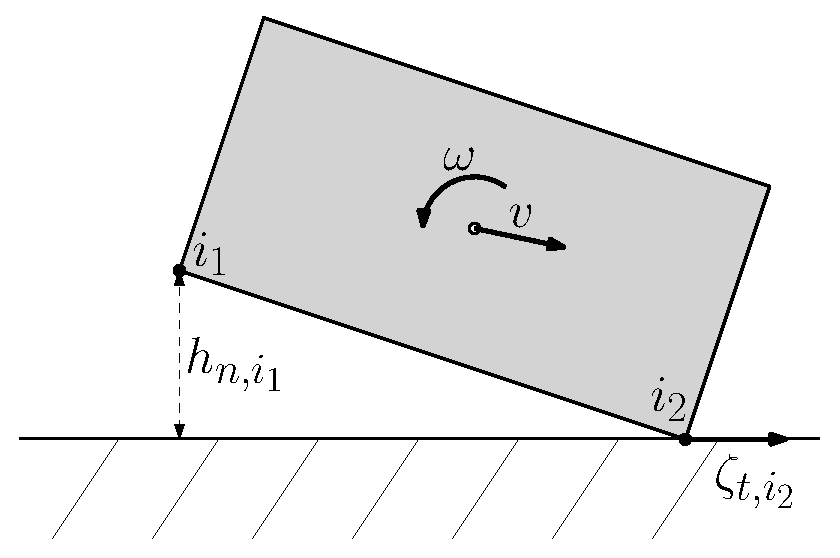
\includegraphics[width=\textwidth]{example2.eps}
\caption{$i_2\in\Ic_{\text{sl}}$}
\label{fig:2example2}
\end{subfigure}
\quad
\begin{subfigure}[b]{0.17\textwidth}   
\centering 
\includegraphics[width=\textwidth]{example3.eps}
\caption{$i_1,i_2\in\Ic_{\text{sl}}$}
\label{fig:2example3}
\end{subfigure}
\quad
\begin{subfigure}[b]{0.17\textwidth}  
\centering 
\includegraphics[width=\textwidth]{example4.eps}
\caption{$i_1\in\Ic_{\text{sl}}$}
\label{fig:2example4}
\end{subfigure}
\quad
\begin{subfigure}[b]{0.17\textwidth}   
\centering 
\includegraphics[width=\textwidth]{example5.eps}
\caption{$i_1,i_2\in\Ic_{\text{op}}$}
\label{fig:2example5}
\end{subfigure}
\vskip\baselineskip
\begin{subfigure}[b]{\textwidth}   
\centering 
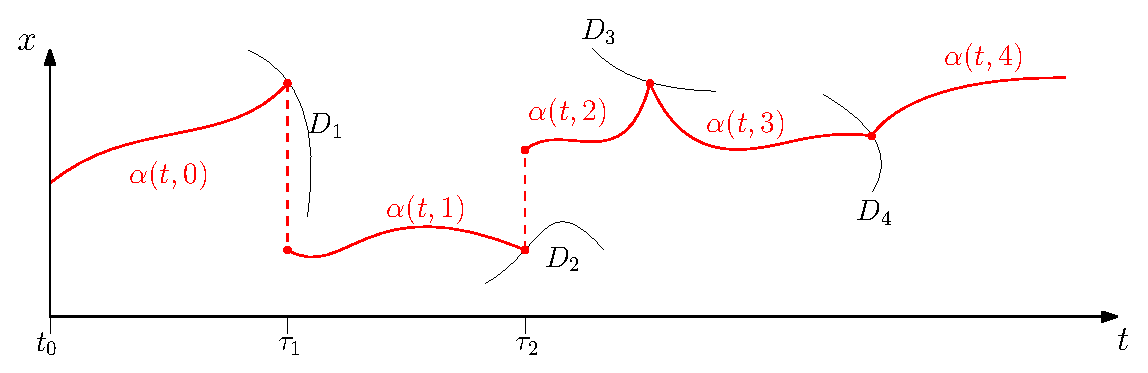
\includegraphics[width=.85\textwidth]{exampletraj1.eps}
\caption{The state-trajectory of a block pushing towards a surface, then sliding across that surface and finally releasing from the surface.}
\label{fig:2exampletraj}
\end{subfigure}
\caption{An example trajectory, which satisfies the dynamics \eqref{eq:hybimp}, of a block pushing towards and withdrawing from a surface with velocity $v$.  Note that the sets $D$ besides being dependent on $\xb$, are also dependent on $\ub$. Also, although not depicted in this image, the state space of the system varies with every event.}
\label{fig:2example}
\end{figure}

The following sections will be used to write the complementarity system defined in Section~\ref{sec:comp} into a hybrid system with impulsive effects as in \eqref{eq:hybimp}. In \ref{sec:2contdyn} the continuous dynamics $\fb_i$ will be derived for mechanical systems with unilateral constraints and spatial friction. Then, in Section~\ref{sec:2event} the reset set $D_i$ will be defined. Finally, in Section~\ref{sec:2discdyn} the discrete dynamics $\gb_i$ will be derived. This will fully define the hybrid system with impulsive effects formulation of mechanical systems with unilateral constraints and spatial friction.

\subsection{Continuous dynamics}\label{sec:2contdyn}
When describing mechanical systems, we take 

\begin{align}
\xb = \begin{bmatrix}
\qb\\ \dot{\qb}
\end{bmatrix},\quad
\dot{\xb} = \begin{bmatrix}
\dot{\qb}\\ \ddot{\qb}
\end{bmatrix},
\end{align}

where $\qb$ and $\dot{\qb}$ are the joint positions, velocities and accelerations respectively. As described in Section~\ref{sec:comp}, for mechanical systems a set of contact points $\iota\in\{\iota_1,\iota_2,...,\iota_c\}$ is defined. Here $c$ is the number of considered contact points. A set $\Ic_{\text{cl}}$ is defined as the set of closed contact points, such that a contact $i\in\Ic_{\text{cl}}$ has closed a unilateral constraint. The set of contact points in open contact is defined as $\Ic_{\text{op}} := \{\iota\ |\ \iota\notin\Ic_{\text{cl}}\}$. The set $\Ic_{\text{cl}}$ is subdivided in two subsets $\Ic_{\text{sl}}$ and $\Ic_{\text{st}}$, where $\Ic_{\text{sl}}$ is the set of closed contact points in slip and $\Ic_{\text{st}}$ the set of closed contact points in stick. Here $\Ic_{\text{cl}} =\Ic_{\text{sl}}\cup\Ic_{\text{st}}$ and $\Ic_{\text{sl}}\cup\Ic_{\text{st}}=\emptyset$. 

The equations of motion, given in \eqref{eq:appcont1}, can be rewritten to
\begin{align}
\ddot{\qb} = \Mb^{-1}(\qb)\left[ \Sb(\qb)\ub - \Cb(\qb,\dot{\qb}) + \Wb_{n}(\qb)\lambdab_{n} + \Wb_{t}(\qb)\lambdab_{t}\right],\label{eq:qddot}
\end{align}
with
\begin{align}
\Wb_n &= \begin{bmatrix}
\wb_{n,i_1},\wb_{n,i_2},...,\wb_{n,\iota}
\end{bmatrix}\in\Rbb^{n\times c},\\
\Wb_t &= \begin{bmatrix}
\Wb_{t,i_1},\Wb_{t,i_2},...,\Wb_{t,\iota} 
\end{bmatrix}\in\Rbb^{n\times 2c},\\
\lambdab_n &= \begin{bmatrix}
\lambda_{n,\iota_1};\lambda_{n,\iota_2};...;\lambda_{n,\iota_c} 
\end{bmatrix}\in\Rbb^{c},\\
\lambdab_t &= \begin{bmatrix}
\lambdab_{t,\iota_1};\lambdab_{t,\iota_2};...;\lambdab_{t,\iota_c} 
\end{bmatrix}\in\Rbb^{2c},
\end{align}
Note that since $\fb_i$ is only defined on $\xb(t,i),\ub(t,i)\notin D_i$, it is not necessary to use $\xib$ to define the equations of motion as done in \eqref{eq:appcont1}. Now $\fb_i$ can be written as
\begin{align}
\dot{\xb}(t,i) =\begin{bmatrix}
\dot{\qb}\\ \Mb^{-1}(\qb)\left[ \Sb(\qb)\ub - \Cb(\qb,\dot{\qb}) + \Wb_{n}(\qb)\lambdab_{n} + \Wb_{t}(\qb)\lambdab_{t}\right]
\end{bmatrix}.\label{eq:fcont}
\end{align}
The closed contact points in $\Ic_{\text{cl}}$ experience reaction forces $\lambda_{n,\iota}$ and $\lambdab_{t,\iota}$, as can be seen in \eqref{eq:qddot}. Therefore for all closed contact points $\iota\in\Ic_{\text{cl}}$ constraints are given which define these reaction forces. These constraints are given by
\begin{equation}
\begin{array}{ll}
\wb^T_{n,\iota}(\qb)\ddot{\qb} + \dot{\wb}^T_{n,\iota}(\qb)\dot{\qb} = 0, & \forall \iota\in\Ic_{\text{cl}},\\
\lambdab_{t,\iota} + \mu_{\iota}\lambda_{n,\iota}\SgnSp(\Wb_{t,\iota}^T\dot{\qb}) = 0, & \forall \iota\in\Ic_{\text{sl}},\\
\Wb^T_{t,\iota}(\qb)\ddot{\qb} + \dot{\Wb}^T_{t,\iota}(\qb)\dot{\qb} = 0, & \forall \iota\in\Ic_{\text{st}},
\end{array}\label{eq:fcontconst}
\end{equation}
where $\Ic_{\text{sl}}$ and $\Ic_{\text{st}}$ are the sets of closed contacts in slip and closed contacts in stick respectively. Now, with \eqref{eq:fcont} and \eqref{eq:fcontconst}, the continuous dynamics of the hybrid system with impulsive dynamics are correctly defined. A more thorough derivation of these dynamics can be found in Appendix~\ref{app:hybrid}.

\subsection{Discrete event sets}\label{sec:2event}
When the continuous dynamics enter an event set $D$, an event will take place. Such an event can cause a contact point to enter a different set. This will lead to different post-event continuous dynamics, and it can cause the state to reinitialize according to the discrete dynamics presented in Section~\ref{sec:2discdyn}. For each set of contact points these sets are defined differently. In this section the sets $D$ are defined for each set of contact points. The derivation of the discrete event sets can be found in Appendix~\ref{app:hybrid}.

\textbf{Discrete events sets in open contact}\\
For all contact points $\iota\in\Ic_{\text{op}}$ the discrete event sets are defined as
\begin{align}
D^{\text{op}\rightarrow\text{cl}}_{\iota} &= \{ \qb\ |\ \gamma^{\text{op}\rightarrow\text{cl}}_{\iota} = 0,\ \dot{\gamma}^{\text{op}\rightarrow\text{cl}}_{\iota} < 0 \},\label{eq:2Dopcl}
\end{align}
with
\begin{align}
\gamma^{\text{op}\rightarrow\text{cl}}_{\iota} &= h_{n,\iota}(\qb),
\end{align}
This event set leads to an impulsive event, which is described in Section~\ref{sec:2discdyn}.

\textbf{Discrete events sets in closed contact slip}\\
For all contact points $\iota\in\Ic_{\text{sl}}$ the discrete event sets are defined as
\begin{align}
D^{\text{sl}\rightarrow\text{st}}_{\iota} &= \{ \qb\ |\ \gamma^{\text{sl}\rightarrow\text{st}}_{\iota} = 0,\ \dot{\gamma}^{\text{sl}\rightarrow\text{st}}_{\iota} < 0\},\label{eq:2Dslst}\\
D^{\text{sl}\rightarrow\text{op}}_{\iota} &= \{ \qb,\ub\ |\ \gamma^{\text{cl}\rightarrow\text{op}}_{\iota} = 0,\ \dot{\gamma}^{\text{cl}\rightarrow\text{op}}_{\iota} < 0\},\label{eq:2Dslop}
\end{align}
with 
\begin{align}
\gamma^{\text{sl}\rightarrow\text{st}}_{\iota} &= \zetab_{t,\iota}\zetab_{t,\iota}^T\\
\gamma^{\text{cl}\rightarrow\text{op}}_{\iota} &= \lambda_{n,\iota}.
\end{align}
These event sets lead to a non-impulsive event, which is described in Section~\ref{sec:2discdyn}.

\textbf{Discrete events sets in closed contact stick}\\
For all contact points $\iota\in\Ic_{\text{st}}$ the discrete event sets are defined as
\begin{align}
D^{\text{st}\rightarrow\text{sl}}_{\iota} &= \{ \qb,\ub\ |\ \gamma^{\text{st}\rightarrow\text{sl}}_{\iota} = 0,\ \dot{\gamma}^{\text{sl}\rightarrow\text{st}}_{\iota} < 0\},\label{eq:2Dstsl}\\
D^{\text{st}\rightarrow\text{op}}_{\iota} &= \{ \qb,\ub\ |\ \gamma^{\text{cl}\rightarrow\text{op}}_{\iota} = 0,\ \dot{\gamma}^{\text{cl}\rightarrow\text{op}}_{\iota} < 0\},\label{eq:2Dstop}
\end{align}
with 
\begin{align}
\gamma^{\text{st}\rightarrow\text{sl}}_{\iota} &= \mu^2\lambda_{n,\iota}^2-\lambdab_{t,\iota}\lambdab_{t,\iota}^T\\
\gamma^{\text{cl}\rightarrow\text{op}}_{\iota} &= \lambda_{n,\iota}.
\end{align}
These event sets lead to a non-impulsive event, which is described in Section~\ref{sec:2discdyn}.

\subsection{Discrete dynamics}\label{sec:2discdyn}
When a contact point enters a discrete event set $D$, the system goes through an event. Since the state can be reinitialized during such an event, the event can cause other contact points to experience infeasible reaction forces. This means that one contact point entering a discrete event set can cause other contact points to enter a discrete event set, making it difficult to determine what the mode of the system after the event will be. The reinitialization of the state and selection of a post-event mode is described by the discrete dynamics in this section. The discrete dynamics for both impulsive and non-impulsive events are described in this section. Since it is unknown before an event what the post-event mode is, a mode selection algorithm is presented to find a feasible post-event mode. This feasible post-event mode can also be found by solving the NCP defined in Section~\ref{sec:comp}. This NCP generates a unique feasible solution \cite{Delassus1917}, which for simple systems can be found by iterating over all solutions until the feasible solution is found. The mode selection algorithm presented in this section will find the same unique feasible solution for the hybrid system.
\nomenclature[A]{NCP}{Nonlinear Complementarity Problem}%

\textbf{State reinitialization}\\
During a transition triggered by \eqref{eq:2Dopcl}, the ante-impact position will always be equal to the post-impact position. The ante and post-event velocity can differ however. \textbf{Add that this is a result from adding friction and releasing.} When $\dot{\qb}^+\neq\dot{\qb}^-$ one speaks of an impulsive discontinuity, and when $\dot{\qb}^+=\dot{\qb}^-$ one speaks of a (non-impulsive) Filippov-discontinuity. In the case of mechanical systems, a contact point making contact with a surface at non-zero velocity will result in an impulsive discontinuity. Other events (releasing and stick-slip transitions) will result in a Filippov-discontinuity. No impulsive forces are present in a Filippov-discontinuity. One could also say that an impulsive discontinuity is defined on velocity level, and a Filippov-discontinuity is defined on acceleration level.

From the impulsive dynamics \eqref{eq:ncpimpact1}-\eqref{eq:ncpimpact4}, the discrete dynamics of an impulsive event can be derived as
\begin{align}
\dot{\qb}^+ &= \Mb^{-1}\left[\Wb_{n}\Lambdab_{n} + \Wb_{t}\Lambdab_{t}\right] + \dot{\qb}^-, \label{eq:2imp1}\\
\wb^T_{n,\iota}\dot{\qb}^+ &= 0, &\forall \iota\in\Ic_{\text{cl}},\label{eq:2imp2}\\
\Lambdab_{t,\iota} + \mu\Lambda_{n,\iota}\SgnSp(\zetab^-_{t,\iota})&= 0, &\forall \iota\in\Ic_{\text{sl}},\label{eq:2imp3}\\
\Wb^T_{t,\iota}\dot{\qb}^+ &= 0, &\forall \iota\in\Ic_{\text{st}}.\label{eq:2imp4}
\end{align}
This system has similar dimensions as the non-impulsive dynamics and is therefore also solvable.

An impulsive event is an event at velocity level. This means that guard functions defined at velocity level can change value, and therefore sign, during an impulsive event. The guard functions that determine the feasibility in an impulsive event are
\begin{align}
\Gamma^{\text{cl}\rightarrow\text{op}}_{\iota}(\dot{\qb}) &= \Lambda_{n,\iota},\\
\Gamma^{\text{sl}\rightarrow\text{st}}_{\iota}(\dot{\qb}) &= \zetab_{t,\iota}\zetab_{t,\iota}^T,\\
\Gamma^{\text{st}\rightarrow\text{sl}}_{\iota}(\dot{\qb}) &= \mu^2\Lambda_{n,\iota}^2 - \Lambdab_{t,\iota}\Lambdab_{t,\iota}^T.
\end{align}
Again, contact points in open contact can only activate position level guard and therefore need not to be considered.

\textbf{Mode selection}\\
The problem that remains is that it is not straightforward to know which dynamics to solve, because the dynamics change as the post-impact mode changes. The dynamics that should be solved are the dynamics that correspond to the post-impact mode which generates a feasible post-impact state. When a contact point enters a discrete event set, and thus generates an infeasible state, it can be concluded that the system will go through an event because in it's current mode the system is infeasible. However, it is not guaranteed that the contact point which entered the event set will change their mode. Actually any contact point, or even several contact points, can change their mode. Therefore the dynamics should be solved for several modes, until a feasible post-event state is found. A feasible post-event state is a post-impact state solved for a certain set of modes of $\iota$, such that the all corresponding guard functions are in its unactivated state, i.e., all $\gamma$ for that mode should be greater than zero. As mentioned earlier, there will exist a unique post-impact mode where the system has a feasible post-impact state. This process where a feasible post-event is found is called \textit{mode selection}.

From the continuous dynamics \eqref{eq:ncpcontact1}-\eqref{eq:ncpcontact4}, the discrete dynamics of a non-impulsive event can be derived as
\begin{align}
\ddot{\qb}^+ &= \Mb^{-1}\left[\Sb\ub^+ - \Cb + \Wb_{n}\lambdab^+_{n} + \Wb_{t}\lambdab^+_{t}\right], &  \label{eq:2nonimp1}\\
\wb^T_{n,\iota}\ddot{\qb}^+ + \dot{\wb}^T_{n,\iota}\dot{\qb}^+ &= 0, & \forall \iota\in\Ic_{\text{cl}},\label{eq:2nonimp2}\\
\lambdab^+_{t,\iota} + \mu\lambda^+_{n,\iota}\SgnSp(\Wb_{t,\iota}^T\dot{\qb}^+) &= 0, & \forall \iota\in\Ic_{\text{sl}},\label{eq:2nonimp3}\\
\Wb^T_{t,\iota}\ddot{\qb}^+ + \dot{\Wb}^T_{t,\iota}\dot{\qb}^+ &= 0, & \forall \iota\in\Ic_{\text{st}},\label{eq:2nonimp4}
\end{align}
where $\Mb$, $\Sb$, $\Cb$, $\wb_{n,\iota}$ and $\Wb_{t,\iota}$ are evaluated at the post-event state $\qb^+$ and state time-derivative $\dot{\qb}^+$. Here the unknown variables are $\ddot{\qb}^+\in\Rbb^{n}$, $\lambdab_{n}\in\Rbb^{c_{\text{cl}}}$ and $\lambdab_{t}\in\Rbb^{2c_{\text{cl}}}$, which means that there are $n+3c_{\text{cl}}$ unknown variables. From \eqref{eq:2nonimp1} we get $n$ equations, from \eqref{eq:2nonimp2} we get $c_{\text{cl}}$ equations and since $\Ic_{\text{sl}}\cup\Ic_{\text{st}}=\Ic_{\text{cl}}$, $\lambdab_{t,\iota}\in\Rbb^2$, and $\Wb^T_{t,\iota}\ddot{\qb}^+ + \dot{\Wb}^T_{t,\iota}\dot{\qb}^+ \in\Rbb^2$ we get $2c_{\text{cl}}$ equations from \eqref{eq:2nonimp3}-\eqref{eq:2nonimp4}. Since we have $n+3c_{\text{cl}}$ unknown variables and $n+3c_{\text{cl}}$ equations, the system is solvable.

A non-impulsive event is an event at acceleration level, as can be seen in \eqref{eq:2nonimp1}. This means that guard functions defined on acceleration level can change in value through non-impulsive events. If the guard function changes sign then the system is in an infeasible mode. The guard functions that determine the feasibility of a non-impulsive event are given by
\begin{align}
\gamma^{\text{cl}\rightarrow\text{op}}_{\iota}(\ddot{\qb}) &= \lambda_{n,\iota}, & \forall \iota\in\Ic_{\text{cl}},\\
\gamma^{\text{st}\rightarrow\text{sl}}_{\iota}(\ddot{\qb}) &= \mu_{\iota}^2\lambda_{n,\iota}^2 - \lambdab_{t,\iota}\lambdab_{t,\iota}^T, & \forall \iota\in\Ic_{\text{st}},
\end{align}
with $\Ic_{\text{sl}}\cup\Ic_{\text{st}}=\Ic_{\text{cl}}$. When a guard function is larger than zero, it means that the corresponding contact point is experiencing feasible reaction forces. When all guard functions are greater than zero, it means that all contact points are experiencing feasible reaction forces and therefore the post-event mode is feasible. Note that the guard functions for contact points in open contact are undefined. This is unnecessary, because contact points in open contact can only activate guard functions defined at position level. Since the non-impulsive dynamics only update the acceleration, it is impossible for a contact point in open contact to change mode during an impulsive event. This also holds for the guard function from slip to stick, which is defined on velocity level. The guard functions given above are all defined on acceleration level, and therefore can change value during a non-impulsive event.
\nomenclature[V]{$\sigma_i$}{The system-mode descriptor of event $i$}%

That the post-event state that is a result from the impulsive event is determined on velocity level, also means that the acceleration is free in this case. That means that the post-event accelerations of an impulsive event can instantly trigger a non-impulsive event guard. The post-event mode therefore should instantly go through a non-impulsive mode selection to find the correct post-event mode. This is illustrated in Figure~\ref{fig:2eventflowchart}.

\begin{figure}[h]
\centering
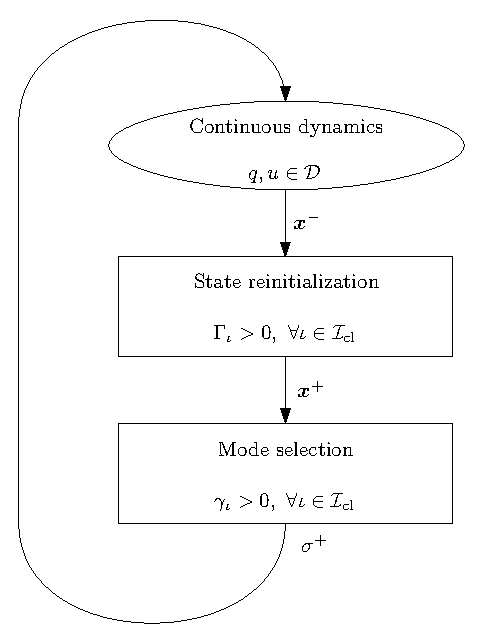
\includegraphics[width=.5\textwidth]{hybridalg.eps}\caption{} \label{fig:2hybridalg}
\end{figure}

\section{Summary}
The modeling of mechanical systems with unilateral constraints and spatial friction is presented in this chapter. First a complementarity problem formulation of such systems is presented, using Signorini's contact law, Poisson's impact law and Coulomb's friction law. This system fully defines the dynamics of mechanical systems with unilateral constraints and spatial friction. From the complementarity problem formulation a hybrid system with impulsive effects is derived. This system is defined with a control point-of-view in mind, and its compatibility with the control strategy that will be presented in the following chapters. The hybrid system is defined in three parts. First the continuous dynamics are presented. Then the discrete event sets are given, which are state-input sets that trigger a discrete event when the state and input enters such a set. Finally the dynamics of such an event are presented, which consist of a state reinitialization and a change in flow dynamics.
\end{document}